\section{Introdução}

Começamos este trabalho apresentando o cenário atual de cursos em ciência de dados (Seção~\ref{sec:ds}), seguido da tendência mundial em adotar currículos baseados em habilidades e competências (Seção~\ref{sec:hc}) para, finalmente, mostrarmos como esses tópicos unem-se para motivar este trabalho (Seção~\ref{sec:motivação})

\subsection{Ciência de dados}\label{sec:ds}

De acordo com o \foreign{National Institute of Standards and Technology} (NIST), ciência de dados (\foreign{data science}, DS) refere-se à atividade de extrair conhecimento acionável de conjuntos de dados brutos utilizando processos de exploração ou formulação e teste de hipóteses \cite[p.~7]{NBDIF2015}.
Ela incorpora princípios, técnicas e métodos de diversas áreas, como ciências da computação, matemática e estatística, além de domínio da área de aplicação.

Essa área tem ganhado notorieade desde o início deste século devido ao crescimento exponencial na geração de dados, conhecido genericamente como \foreign{Big Data}, devido principalmente ao advento da Web 2.0, por volta de 2005, e dos dispositivos móveis, em 2007.
Desde então e também devido ao aumento na capacidade computacional, novas técnicas de análise, a maioria computacionais, tem sido empregadas.
Exemplos notáveis são as redes neurais e a inferência bayesiana.

Nos últimos anos, inúmeras ferramentas robustas de computação e análise de dados, disponibilizadas livremente, têm tornado a ciência de dados cada vez mais acessível \cite{Hayes2019}.
Exemplos são as linguagens de programação Scala \cite{Bugnion2016}, Python (e suas bibliotecas de análise de dados) \cite{Nagpal2019, McKinney2013}, R \cite{James2013} e, mais recentemente, Julia \cite{McNicholas2019}.
Isso sem mencionar a abordagem AutoML, que oferece interfaces simples para o emprego de aprendizagem de máquina sem a necessidade de programação \cite{He2020}.

A facilidade de acesso e a alta demanda por cientistas de dados levou, então, à oferta de cursos de ciência de dados \cite{Hassan2019}: no Brasil, algumas universidades, como a Univesp, a USP e a FIAP, já oferecem cursos de graduação e pós-graduação.
Mas também é possível estudar gratuitamente pela Internet, nas plataformas MOOC (\foreign{Massive Open Online Courses}) como Coursera (\url{coursera.org}), EdX (\url{edx.org}) \etc.

Há também cursos livres nessa área, que ganham força devido ao reconhecimento de que as universidades tradicionais já não suprem a necessidade de mão de obra qualificada em várias áreas \cite{Zulauf2006}.
Esses cursos oferecem uma formação rápida, que varia em torno de um semestre, e visam colocar o candidato no mercado de trabalho independentemente da sua área de formação.
Consulte, por exemplo, os cursos de \foreign{Data Analytics} e \foreign{Data Science} da Digital House (\url{digitalhouse.com/br}) e da Tera (\url{somostera.com}).

\begin{figure}
	\centering

	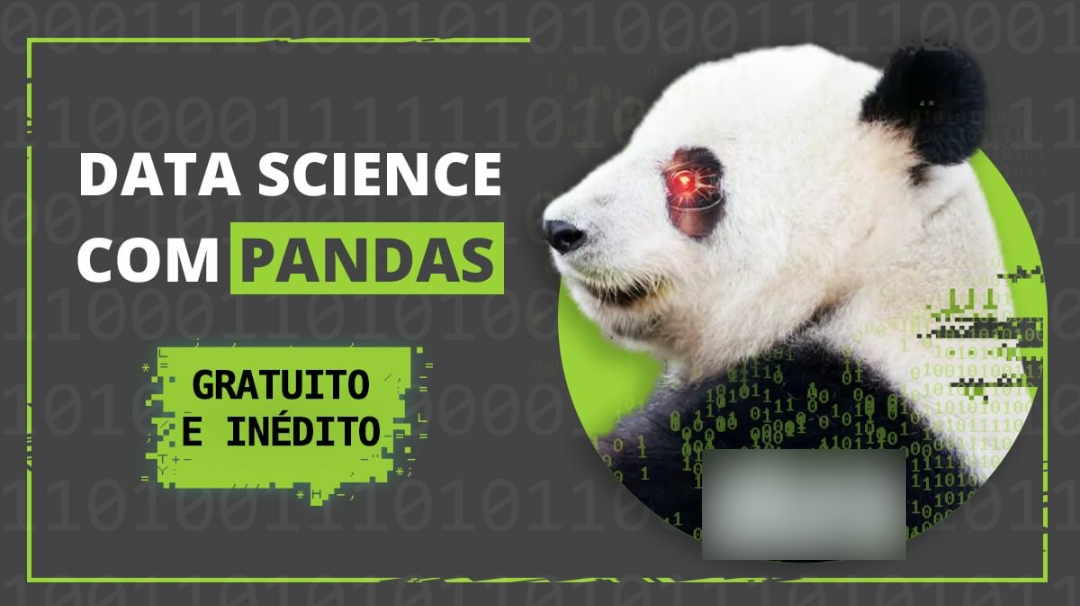
\includegraphics[width=0.45\textwidth]{eg_ds_1}\hfill
	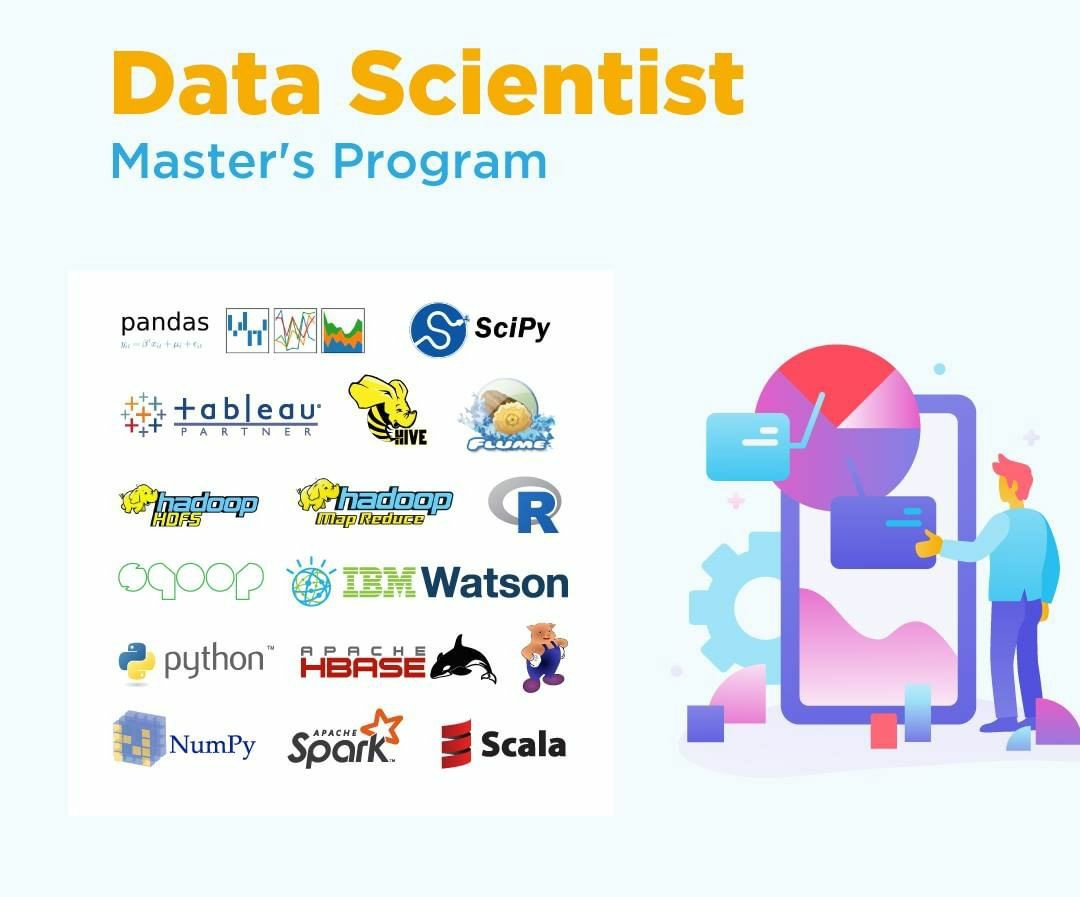
\includegraphics[width=0.45\textwidth]{eg_ds_2}

	\caption{Anúncios de cursos livres de ciência de dados.}
	\label{fig:cursos}
\end{figure}

Porém, como esses cursos visam o mercado de trabalho, em geral a divulgação deles enfatiza não os conhecimentos, competências e habilidades que um cientista de dados precisa, mas sim as ferramentas e algoritmos utilizados por eles e que são frequentemente mencionados em vagas de de emprego.

A Figura~\ref{fig:cursos} ilustra isso: ela apresenta a propaganda de dois cursos, oferecidos na rede social Instagram.
Em ambos o foco é linguagens de programação (Python, Scala e R), ferramentas de \foreign{Big Data} (Spark, Hadoop \etc), aplicativos (Tableau) e bibliotecas (Pandas, SciPy \etc).

Embora o domínio dessas ferramentas seja necessário, ele não é suficiente para um cientista de dados de fato produzir conhecimento acionável.
Para isso são necessários, por exemplo, métodos de pesquisa, engenharia de dados, inferência estatística, dentre outros \cite[p.~15]{CF-DS-Release2019}.

Argumentamos, então, que a ênfase em ferramentas, linguagens \etc na \emph{divulgação} desses cursos esmorece, aos olhos dos alunos, a importância das habilidades e competências, haja vista que sua relação com as vagas de emprego não são tão explícitas como as linguages e ferramentas.

\subsection{Competências e habilidades}\label{sec:hc}

No Brasil e no mundo, a proposta de substituir os currículos tradicionalmente baseados em conteúdo por aqueles baseados em competências e habilidades tem ganhado força.
Por exemplo, no Brasil a Base Nacional Comum Curricular (BNCC) \cite{BNCC}, homologada em 2018, ``estabelece conhecimentos, competências e habilidades que se espera que todos os estudantes desenvolvam ao longo da escolaridade básica''.
Outros países também seguem a mesma tendência \cite{Inkson2017}.

Essa abordagem tem sido adotada no ensino básico \cite{Avila2017} e superior para direcionar a ``educação brasileira para a formação humana integral e para a construção de uma sociedade justa, democrática e inclusiva''.
De fato, essa abordagem visa a empregabilidade \cite{Voorhees2001}, que é também o objetivo dos cursos livres anteriormente mencionados.

Por exemplo, segundo o \foreign{EDISON Data Science Framework} \cite{CF-DS-Release2019}, algumas competências de um cientista de dados são:
\begin{compactitem}
	\item ``Usar de engenharia (geral e de software) para pesquisar, projetar, desenvolver e implementar novos instrumentos e aplicações para a coleta de dados, armazenamento, análise e visualização''.
	\item ``Utilizar eficientemente uma variedade de técnicas de análise de dados, como aprendizagem de máquina, mineração de dados, análises prescritivas e preditivas, para análise complexa de dados durante todo o ciclo de vida dos dados''
\end{compactitem}
Ademais, exemplos de habilidades são:
\begin{compactitem}
	\item ``Usar aprendizagem de máquina, tecnologia, algoritmos e ferramentas''
	\item ``Projetar experimentos, desenvolver e implementar processos de coleta de dados''
\end{compactitem}

Entretanto, as empresas frequentemente listam ferramentas e algoritmos como requisitos às vagas de trabalho que publicam, ao invés das competências e habilidades necessárias para o exercício da ciência de dados.
A Figura~\ref{fig:vagas} ilustra duas vagas dessa área, obtidas na plataforma LinkedIn.
Nela podemos ver a menção às mesmas ferramentas e algoritmos oferecidos pelos cursos livres.

\begin{figure}
	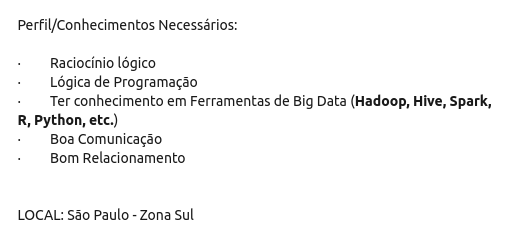
\includegraphics[width=0.45\textwidth]{eg_vaga-1_ds}\hfill
	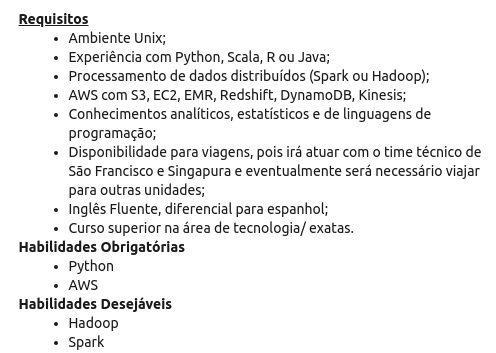
\includegraphics[width=0.45\textwidth]{eg_vaga-2_ds}
	\caption{Duas vagas de cientista de dados, extraídas do LinkedIn.}
	\label{fig:vagas}
\end{figure}

\subsection{Cenário e motivação}\label{sec:motivação}

Em vista do exposto, o autor deste trabalho, que atua como coordenador na instituição educacional Digital House (\url{digitalhouse.com/br}), que por sua vez oferece cursos livres de DS e \foreign{Data Analytics} (DA), gostaria de adotar a aprendizagem baseada em competências nos cursos de ciência de dados e de \foreign{Data Analytics} (DA) sob sua responsabilidade.

Neste trabalho nós analisamos os resultados de aprendizagem nos cursos de DA e DS oferecidos pela instituição educacional mencionada, com o intuito de identificar uma possível concorrência entre os currículos baseados em competências e os incentivos do mercado de trabalho, conforme exposto nas hipóteses deste trabalho (Seção~\ref{sec:hipóteses}).

Conforme a definição de ciência de dados do NIST, os cursos de DA e DS podem ser classificados como de ciência de dados.
Porém, eles guardam semelhanças e diferenças entre si:
\begin{compactitem}
	\item \textbf{\foreign{Data Analytics} (DA):} visa a inteligência de mercado (\foreign{Business Intelligence}, BI), isto é, a aplicação da ciência de dados para obter conhecimento acionável que suporte decisões estratégicas para um empreendimento.
	Esse curso tem carga horária de 140 horas e dura 14 semanas.
	Outra característica desse curso é que ele baseia-se em aplicativos como PowerBI, Tableau, MySQL \etc.

	\item \textbf{\foreign{Data Science} (DS):} visa o desenvolvimento de ``produtos de dados'', isto é, \foreign{softwares} que automaticamente obtém conhecimento acionável para oferecê-lo aos clientes.
	Esse curso tem carga horária de 196 horas, dura 19 semanas e baseia-se na linguagem de programação Python e suas extensões para análise de dados.
\end{compactitem}

A tabela abaixo resume o que foi exposto imediatamente acima, comparando os dois cursos.

{\footnotesize
\noindent%
\begin{tabular}{lllll}
	\toprule
	Curso & Objetivo & \shortstack[l]{Carga\\horária (horas)} & \shortstack[c]{Duração\\(semanas)} & Ferramenta\\
	\midrule
	DA & Inteligência de mercado & 140 & 14 & Aplicativos\\
	DS & Produto de dados & 196 & 19 & Linguagem de programação	\\
	\bottomrule
\end{tabular}
}